\documentclass{article}
\usepackage[utf8]{inputenc}
\usepackage{tikz}
\usetikzlibrary{automata}

\usepackage{float}
\begin{document}
\title{Übungsaufgaben}
\author{Simon Stroh und Moritz von Looz}
\maketitle
\section{Endliche Automaten}
Gegeben sei folgender endlicher Automat:
\begin{figure}[H]
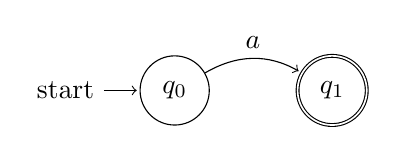
\begin{tikzpicture}[node distance=2cm,shorten >=1pt,auto]
\node[state,initial] 	(q_0)			{$q_0$};
\node[state,accepting]	(q_1)	[right of=q_0]	{$q_1$};
\path[->]		(q_0)	edge [bend left]	node	{$a$}	(q_1);
\end{tikzpicture}
\end{figure}
\begin{enumerate}
\item Bilde einen äquivalenten, minimalen DEA.
\item Was sind die Äquivalenzklassen für diesen Automaten bezüglich der Neroderelation?
\item Bilde einen Regulären Ausdruck der die gleiche Sprache akzeptiert wie der Automat.
\end{enumerate}
\section{Pumping Lemma}
Zeige oder Wiederlege die regulärität folgender Sprachen:
\begin{enumerate}
\item TODO 
\item TODO
\end{enumerate}
\section{Turingmaschinen}
\begin{enumerate}
\item TODO %was mit Gödelnummern
\item TODO %TM varianten
\end{enumerate}
\section{Entscheidbarkeit}
\begin{enumerate}
\item TODO %Nichtentscheidbare Sprachen
\item TODO %Halteproblem
\item TODO %Rice
\item TODO %PCP
\item TODO %Semientscheidbare
\end{enumerate}
\section{Komplexitätsklassen}
\begin{enumerate}
\item TODO %NDTM
\item TODO %Kodierungsschemata
\item TODO %NP & NPC
\end{enumerate}
\end{document}
